% Created by tikzDevice version 0.12.6 on 2025-02-15 06:19:01
% !TEX encoding = UTF-8 Unicode
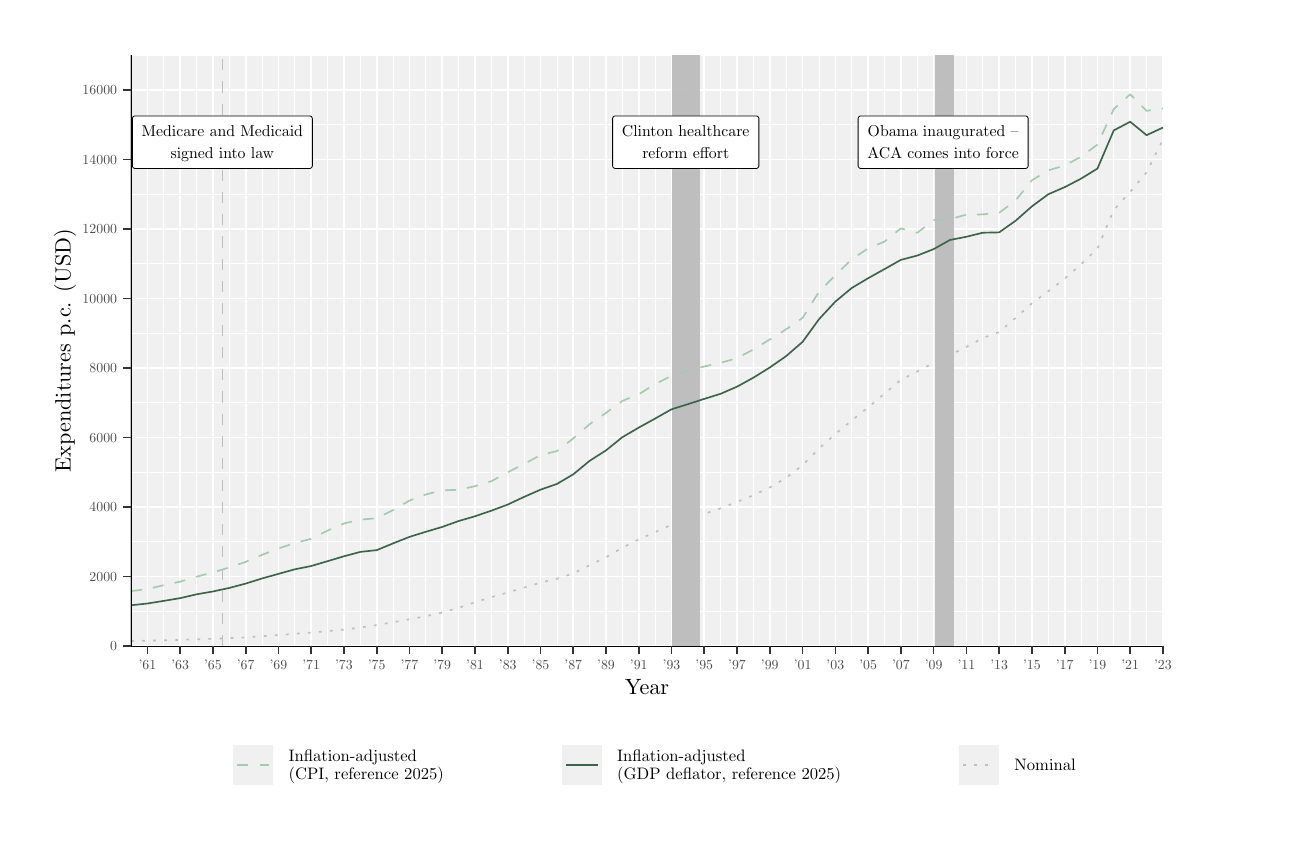
\begin{tikzpicture}[x=1pt,y=1pt]
\definecolor{fillColor}{RGB}{255,255,255}
\path[use as bounding box,fill=fillColor,fill opacity=0.00] (0,0) rectangle (455.30,289.08);
\begin{scope}
\path[clip] (  0.00,  0.00) rectangle (455.30,289.08);
\definecolor{drawColor}{RGB}{255,255,255}
\definecolor{fillColor}{RGB}{255,255,255}

\path[draw=drawColor,line width= 0.6pt,line join=round,line cap=round,fill=fillColor] ( -0.00,  0.00) rectangle (455.30,289.08);
\end{scope}
\begin{scope}
\path[clip] (  0.00,  0.00) rectangle (455.30,289.08);
\definecolor{fillColor}{gray}{0.94}

\path[fill=fillColor] ( 37.26, 65.63) rectangle (410.30,279.08);
\definecolor{drawColor}{RGB}{255,255,255}

\path[draw=drawColor,line width= 0.3pt,line join=round] ( 37.26, 78.19) --
	(410.30, 78.19);

\path[draw=drawColor,line width= 0.3pt,line join=round] ( 37.26,103.30) --
	(410.30,103.30);

\path[draw=drawColor,line width= 0.3pt,line join=round] ( 37.26,128.41) --
	(410.30,128.41);

\path[draw=drawColor,line width= 0.3pt,line join=round] ( 37.26,153.52) --
	(410.30,153.52);

\path[draw=drawColor,line width= 0.3pt,line join=round] ( 37.26,178.64) --
	(410.30,178.64);

\path[draw=drawColor,line width= 0.3pt,line join=round] ( 37.26,203.75) --
	(410.30,203.75);

\path[draw=drawColor,line width= 0.3pt,line join=round] ( 37.26,228.86) --
	(410.30,228.86);

\path[draw=drawColor,line width= 0.3pt,line join=round] ( 37.26,253.97) --
	(410.30,253.97);

\path[draw=drawColor,line width= 0.3pt,line join=round] ( 37.26,279.08) --
	(410.30,279.08);

\path[draw=drawColor,line width= 0.3pt,line join=round] ( 37.35, 65.63) --
	( 37.35,279.08);

\path[draw=drawColor,line width= 0.3pt,line join=round] ( 49.19, 65.63) --
	( 49.19,279.08);

\path[draw=drawColor,line width= 0.3pt,line join=round] ( 61.03, 65.63) --
	( 61.03,279.08);

\path[draw=drawColor,line width= 0.3pt,line join=round] ( 72.86, 65.63) --
	( 72.86,279.08);

\path[draw=drawColor,line width= 0.3pt,line join=round] ( 84.70, 65.63) --
	( 84.70,279.08);

\path[draw=drawColor,line width= 0.3pt,line join=round] ( 96.54, 65.63) --
	( 96.54,279.08);

\path[draw=drawColor,line width= 0.3pt,line join=round] (108.37, 65.63) --
	(108.37,279.08);

\path[draw=drawColor,line width= 0.3pt,line join=round] (120.21, 65.63) --
	(120.21,279.08);

\path[draw=drawColor,line width= 0.3pt,line join=round] (132.05, 65.63) --
	(132.05,279.08);

\path[draw=drawColor,line width= 0.3pt,line join=round] (143.89, 65.63) --
	(143.89,279.08);

\path[draw=drawColor,line width= 0.3pt,line join=round] (155.72, 65.63) --
	(155.72,279.08);

\path[draw=drawColor,line width= 0.3pt,line join=round] (167.56, 65.63) --
	(167.56,279.08);

\path[draw=drawColor,line width= 0.3pt,line join=round] (179.40, 65.63) --
	(179.40,279.08);

\path[draw=drawColor,line width= 0.3pt,line join=round] (191.24, 65.63) --
	(191.24,279.08);

\path[draw=drawColor,line width= 0.3pt,line join=round] (203.07, 65.63) --
	(203.07,279.08);

\path[draw=drawColor,line width= 0.3pt,line join=round] (214.91, 65.63) --
	(214.91,279.08);

\path[draw=drawColor,line width= 0.3pt,line join=round] (226.75, 65.63) --
	(226.75,279.08);

\path[draw=drawColor,line width= 0.3pt,line join=round] (238.58, 65.63) --
	(238.58,279.08);

\path[draw=drawColor,line width= 0.3pt,line join=round] (250.42, 65.63) --
	(250.42,279.08);

\path[draw=drawColor,line width= 0.3pt,line join=round] (262.26, 65.63) --
	(262.26,279.08);

\path[draw=drawColor,line width= 0.3pt,line join=round] (274.10, 65.63) --
	(274.10,279.08);

\path[draw=drawColor,line width= 0.3pt,line join=round] (285.93, 65.63) --
	(285.93,279.08);

\path[draw=drawColor,line width= 0.3pt,line join=round] (297.77, 65.63) --
	(297.77,279.08);

\path[draw=drawColor,line width= 0.3pt,line join=round] (309.61, 65.63) --
	(309.61,279.08);

\path[draw=drawColor,line width= 0.3pt,line join=round] (321.44, 65.63) --
	(321.44,279.08);

\path[draw=drawColor,line width= 0.3pt,line join=round] (333.28, 65.63) --
	(333.28,279.08);

\path[draw=drawColor,line width= 0.3pt,line join=round] (345.12, 65.63) --
	(345.12,279.08);

\path[draw=drawColor,line width= 0.3pt,line join=round] (356.96, 65.63) --
	(356.96,279.08);

\path[draw=drawColor,line width= 0.3pt,line join=round] (368.79, 65.63) --
	(368.79,279.08);

\path[draw=drawColor,line width= 0.3pt,line join=round] (380.63, 65.63) --
	(380.63,279.08);

\path[draw=drawColor,line width= 0.3pt,line join=round] (392.47, 65.63) --
	(392.47,279.08);

\path[draw=drawColor,line width= 0.3pt,line join=round] (404.31, 65.63) --
	(404.31,279.08);

\path[draw=drawColor,line width= 0.6pt,line join=round] ( 37.26, 65.63) --
	(410.30, 65.63);

\path[draw=drawColor,line width= 0.6pt,line join=round] ( 37.26, 90.75) --
	(410.30, 90.75);

\path[draw=drawColor,line width= 0.6pt,line join=round] ( 37.26,115.86) --
	(410.30,115.86);

\path[draw=drawColor,line width= 0.6pt,line join=round] ( 37.26,140.97) --
	(410.30,140.97);

\path[draw=drawColor,line width= 0.6pt,line join=round] ( 37.26,166.08) --
	(410.30,166.08);

\path[draw=drawColor,line width= 0.6pt,line join=round] ( 37.26,191.19) --
	(410.30,191.19);

\path[draw=drawColor,line width= 0.6pt,line join=round] ( 37.26,216.30) --
	(410.30,216.30);

\path[draw=drawColor,line width= 0.6pt,line join=round] ( 37.26,241.41) --
	(410.30,241.41);

\path[draw=drawColor,line width= 0.6pt,line join=round] ( 37.26,266.52) --
	(410.30,266.52);

\path[draw=drawColor,line width= 0.6pt,line join=round] ( 43.27, 65.63) --
	( 43.27,279.08);

\path[draw=drawColor,line width= 0.6pt,line join=round] ( 55.10, 65.63) --
	( 55.10,279.08);

\path[draw=drawColor,line width= 0.6pt,line join=round] ( 66.95, 65.63) --
	( 66.95,279.08);

\path[draw=drawColor,line width= 0.6pt,line join=round] ( 78.78, 65.63) --
	( 78.78,279.08);

\path[draw=drawColor,line width= 0.6pt,line join=round] ( 90.62, 65.63) --
	( 90.62,279.08);

\path[draw=drawColor,line width= 0.6pt,line join=round] (102.45, 65.63) --
	(102.45,279.08);

\path[draw=drawColor,line width= 0.6pt,line join=round] (114.30, 65.63) --
	(114.30,279.08);

\path[draw=drawColor,line width= 0.6pt,line join=round] (126.13, 65.63) --
	(126.13,279.08);

\path[draw=drawColor,line width= 0.6pt,line join=round] (137.97, 65.63) --
	(137.97,279.08);

\path[draw=drawColor,line width= 0.6pt,line join=round] (149.80, 65.63) --
	(149.80,279.08);

\path[draw=drawColor,line width= 0.6pt,line join=round] (161.65, 65.63) --
	(161.65,279.08);

\path[draw=drawColor,line width= 0.6pt,line join=round] (173.48, 65.63) --
	(173.48,279.08);

\path[draw=drawColor,line width= 0.6pt,line join=round] (185.32, 65.63) --
	(185.32,279.08);

\path[draw=drawColor,line width= 0.6pt,line join=round] (197.15, 65.63) --
	(197.15,279.08);

\path[draw=drawColor,line width= 0.6pt,line join=round] (209.00, 65.63) --
	(209.00,279.08);

\path[draw=drawColor,line width= 0.6pt,line join=round] (220.82, 65.63) --
	(220.82,279.08);

\path[draw=drawColor,line width= 0.6pt,line join=round] (232.67, 65.63) --
	(232.67,279.08);

\path[draw=drawColor,line width= 0.6pt,line join=round] (244.50, 65.63) --
	(244.50,279.08);

\path[draw=drawColor,line width= 0.6pt,line join=round] (256.34, 65.63) --
	(256.34,279.08);

\path[draw=drawColor,line width= 0.6pt,line join=round] (268.17, 65.63) --
	(268.17,279.08);

\path[draw=drawColor,line width= 0.6pt,line join=round] (280.02, 65.63) --
	(280.02,279.08);

\path[draw=drawColor,line width= 0.6pt,line join=round] (291.85, 65.63) --
	(291.85,279.08);

\path[draw=drawColor,line width= 0.6pt,line join=round] (303.69, 65.63) --
	(303.69,279.08);

\path[draw=drawColor,line width= 0.6pt,line join=round] (315.52, 65.63) --
	(315.52,279.08);

\path[draw=drawColor,line width= 0.6pt,line join=round] (327.37, 65.63) --
	(327.37,279.08);

\path[draw=drawColor,line width= 0.6pt,line join=round] (339.20, 65.63) --
	(339.20,279.08);

\path[draw=drawColor,line width= 0.6pt,line join=round] (351.04, 65.63) --
	(351.04,279.08);

\path[draw=drawColor,line width= 0.6pt,line join=round] (362.87, 65.63) --
	(362.87,279.08);

\path[draw=drawColor,line width= 0.6pt,line join=round] (374.72, 65.63) --
	(374.72,279.08);

\path[draw=drawColor,line width= 0.6pt,line join=round] (386.55, 65.63) --
	(386.55,279.08);

\path[draw=drawColor,line width= 0.6pt,line join=round] (398.39, 65.63) --
	(398.39,279.08);

\path[draw=drawColor,line width= 0.6pt,line join=round] (410.22, 65.63) --
	(410.22,279.08);
\definecolor{drawColor}{RGB}{190,190,190}

\path[draw=drawColor,line width= 0.6pt,line join=round] ( 37.34, 65.63) -- ( 37.34,279.08);
\definecolor{fillColor}{RGB}{190,190,190}

\path[fill=fillColor,fill opacity=0.01] (232.67, 65.63) rectangle (242.93,279.08);

\path[fill=fillColor,fill opacity=0.01] (232.67, 65.63) rectangle (242.93,279.08);

\path[fill=fillColor,fill opacity=0.01] (232.67, 65.63) rectangle (242.93,279.08);

\path[fill=fillColor,fill opacity=0.01] (232.67, 65.63) rectangle (242.93,279.08);

\path[fill=fillColor,fill opacity=0.01] (232.67, 65.63) rectangle (242.93,279.08);

\path[fill=fillColor,fill opacity=0.01] (232.67, 65.63) rectangle (242.93,279.08);

\path[fill=fillColor,fill opacity=0.01] (232.67, 65.63) rectangle (242.93,279.08);

\path[fill=fillColor,fill opacity=0.01] (232.67, 65.63) rectangle (242.93,279.08);

\path[fill=fillColor,fill opacity=0.01] (232.67, 65.63) rectangle (242.93,279.08);

\path[fill=fillColor,fill opacity=0.01] (232.67, 65.63) rectangle (242.93,279.08);

\path[fill=fillColor,fill opacity=0.01] (232.67, 65.63) rectangle (242.93,279.08);

\path[fill=fillColor,fill opacity=0.01] (232.67, 65.63) rectangle (242.93,279.08);

\path[fill=fillColor,fill opacity=0.01] (232.67, 65.63) rectangle (242.93,279.08);

\path[fill=fillColor,fill opacity=0.01] (232.67, 65.63) rectangle (242.93,279.08);

\path[fill=fillColor,fill opacity=0.01] (232.67, 65.63) rectangle (242.93,279.08);

\path[fill=fillColor,fill opacity=0.01] (232.67, 65.63) rectangle (242.93,279.08);

\path[fill=fillColor,fill opacity=0.01] (232.67, 65.63) rectangle (242.93,279.08);

\path[fill=fillColor,fill opacity=0.01] (232.67, 65.63) rectangle (242.93,279.08);

\path[fill=fillColor,fill opacity=0.01] (232.67, 65.63) rectangle (242.93,279.08);

\path[fill=fillColor,fill opacity=0.01] (232.67, 65.63) rectangle (242.93,279.08);

\path[fill=fillColor,fill opacity=0.01] (232.67, 65.63) rectangle (242.93,279.08);

\path[fill=fillColor,fill opacity=0.01] (232.67, 65.63) rectangle (242.93,279.08);

\path[fill=fillColor,fill opacity=0.01] (232.67, 65.63) rectangle (242.93,279.08);

\path[fill=fillColor,fill opacity=0.01] (232.67, 65.63) rectangle (242.93,279.08);

\path[fill=fillColor,fill opacity=0.01] (232.67, 65.63) rectangle (242.93,279.08);

\path[fill=fillColor,fill opacity=0.01] (232.67, 65.63) rectangle (242.93,279.08);

\path[fill=fillColor,fill opacity=0.01] (232.67, 65.63) rectangle (242.93,279.08);

\path[fill=fillColor,fill opacity=0.01] (232.67, 65.63) rectangle (242.93,279.08);

\path[fill=fillColor,fill opacity=0.01] (232.67, 65.63) rectangle (242.93,279.08);

\path[fill=fillColor,fill opacity=0.01] (232.67, 65.63) rectangle (242.93,279.08);

\path[fill=fillColor,fill opacity=0.01] (232.67, 65.63) rectangle (242.93,279.08);

\path[fill=fillColor,fill opacity=0.01] (232.67, 65.63) rectangle (242.93,279.08);

\path[fill=fillColor,fill opacity=0.01] (232.67, 65.63) rectangle (242.93,279.08);

\path[fill=fillColor,fill opacity=0.01] (232.67, 65.63) rectangle (242.93,279.08);

\path[fill=fillColor,fill opacity=0.01] (232.67, 65.63) rectangle (242.93,279.08);

\path[fill=fillColor,fill opacity=0.01] (232.67, 65.63) rectangle (242.93,279.08);

\path[fill=fillColor,fill opacity=0.01] (232.67, 65.63) rectangle (242.93,279.08);

\path[fill=fillColor,fill opacity=0.01] (232.67, 65.63) rectangle (242.93,279.08);

\path[fill=fillColor,fill opacity=0.01] (232.67, 65.63) rectangle (242.93,279.08);

\path[fill=fillColor,fill opacity=0.01] (232.67, 65.63) rectangle (242.93,279.08);

\path[fill=fillColor,fill opacity=0.01] (232.67, 65.63) rectangle (242.93,279.08);

\path[fill=fillColor,fill opacity=0.01] (232.67, 65.63) rectangle (242.93,279.08);

\path[fill=fillColor,fill opacity=0.01] (232.67, 65.63) rectangle (242.93,279.08);

\path[fill=fillColor,fill opacity=0.01] (232.67, 65.63) rectangle (242.93,279.08);

\path[fill=fillColor,fill opacity=0.01] (232.67, 65.63) rectangle (242.93,279.08);

\path[fill=fillColor,fill opacity=0.01] (232.67, 65.63) rectangle (242.93,279.08);

\path[fill=fillColor,fill opacity=0.01] (232.67, 65.63) rectangle (242.93,279.08);

\path[fill=fillColor,fill opacity=0.01] (232.67, 65.63) rectangle (242.93,279.08);

\path[fill=fillColor,fill opacity=0.01] (232.67, 65.63) rectangle (242.93,279.08);

\path[fill=fillColor,fill opacity=0.01] (232.67, 65.63) rectangle (242.93,279.08);

\path[fill=fillColor,fill opacity=0.01] (232.67, 65.63) rectangle (242.93,279.08);

\path[fill=fillColor,fill opacity=0.01] (232.67, 65.63) rectangle (242.93,279.08);

\path[fill=fillColor,fill opacity=0.01] (232.67, 65.63) rectangle (242.93,279.08);

\path[fill=fillColor,fill opacity=0.01] (232.67, 65.63) rectangle (242.93,279.08);

\path[fill=fillColor,fill opacity=0.01] (232.67, 65.63) rectangle (242.93,279.08);

\path[fill=fillColor,fill opacity=0.01] (232.67, 65.63) rectangle (242.93,279.08);

\path[fill=fillColor,fill opacity=0.01] (232.67, 65.63) rectangle (242.93,279.08);

\path[fill=fillColor,fill opacity=0.01] (232.67, 65.63) rectangle (242.93,279.08);

\path[fill=fillColor,fill opacity=0.01] (232.67, 65.63) rectangle (242.93,279.08);

\path[fill=fillColor,fill opacity=0.01] (232.67, 65.63) rectangle (242.93,279.08);

\path[fill=fillColor,fill opacity=0.01] (232.67, 65.63) rectangle (242.93,279.08);

\path[fill=fillColor,fill opacity=0.01] (232.67, 65.63) rectangle (242.93,279.08);

\path[fill=fillColor,fill opacity=0.01] (232.67, 65.63) rectangle (242.93,279.08);

\path[fill=fillColor,fill opacity=0.01] (232.67, 65.63) rectangle (242.93,279.08);

\path[fill=fillColor,fill opacity=0.01] (327.68, 65.63) rectangle (334.59,279.08);

\path[fill=fillColor,fill opacity=0.01] (327.68, 65.63) rectangle (334.59,279.08);

\path[fill=fillColor,fill opacity=0.01] (327.68, 65.63) rectangle (334.59,279.08);

\path[fill=fillColor,fill opacity=0.01] (327.68, 65.63) rectangle (334.59,279.08);

\path[fill=fillColor,fill opacity=0.01] (327.68, 65.63) rectangle (334.59,279.08);

\path[fill=fillColor,fill opacity=0.01] (327.68, 65.63) rectangle (334.59,279.08);

\path[fill=fillColor,fill opacity=0.01] (327.68, 65.63) rectangle (334.59,279.08);

\path[fill=fillColor,fill opacity=0.01] (327.68, 65.63) rectangle (334.59,279.08);

\path[fill=fillColor,fill opacity=0.01] (327.68, 65.63) rectangle (334.59,279.08);

\path[fill=fillColor,fill opacity=0.01] (327.68, 65.63) rectangle (334.59,279.08);

\path[fill=fillColor,fill opacity=0.01] (327.68, 65.63) rectangle (334.59,279.08);

\path[fill=fillColor,fill opacity=0.01] (327.68, 65.63) rectangle (334.59,279.08);

\path[fill=fillColor,fill opacity=0.01] (327.68, 65.63) rectangle (334.59,279.08);

\path[fill=fillColor,fill opacity=0.01] (327.68, 65.63) rectangle (334.59,279.08);

\path[fill=fillColor,fill opacity=0.01] (327.68, 65.63) rectangle (334.59,279.08);

\path[fill=fillColor,fill opacity=0.01] (327.68, 65.63) rectangle (334.59,279.08);

\path[fill=fillColor,fill opacity=0.01] (327.68, 65.63) rectangle (334.59,279.08);

\path[fill=fillColor,fill opacity=0.01] (327.68, 65.63) rectangle (334.59,279.08);

\path[fill=fillColor,fill opacity=0.01] (327.68, 65.63) rectangle (334.59,279.08);

\path[fill=fillColor,fill opacity=0.01] (327.68, 65.63) rectangle (334.59,279.08);

\path[fill=fillColor,fill opacity=0.01] (327.68, 65.63) rectangle (334.59,279.08);

\path[fill=fillColor,fill opacity=0.01] (327.68, 65.63) rectangle (334.59,279.08);

\path[fill=fillColor,fill opacity=0.01] (327.68, 65.63) rectangle (334.59,279.08);

\path[fill=fillColor,fill opacity=0.01] (327.68, 65.63) rectangle (334.59,279.08);

\path[fill=fillColor,fill opacity=0.01] (327.68, 65.63) rectangle (334.59,279.08);

\path[fill=fillColor,fill opacity=0.01] (327.68, 65.63) rectangle (334.59,279.08);

\path[fill=fillColor,fill opacity=0.01] (327.68, 65.63) rectangle (334.59,279.08);

\path[fill=fillColor,fill opacity=0.01] (327.68, 65.63) rectangle (334.59,279.08);

\path[fill=fillColor,fill opacity=0.01] (327.68, 65.63) rectangle (334.59,279.08);

\path[fill=fillColor,fill opacity=0.01] (327.68, 65.63) rectangle (334.59,279.08);

\path[fill=fillColor,fill opacity=0.01] (327.68, 65.63) rectangle (334.59,279.08);

\path[fill=fillColor,fill opacity=0.01] (327.68, 65.63) rectangle (334.59,279.08);

\path[fill=fillColor,fill opacity=0.01] (327.68, 65.63) rectangle (334.59,279.08);

\path[fill=fillColor,fill opacity=0.01] (327.68, 65.63) rectangle (334.59,279.08);

\path[fill=fillColor,fill opacity=0.01] (327.68, 65.63) rectangle (334.59,279.08);

\path[fill=fillColor,fill opacity=0.01] (327.68, 65.63) rectangle (334.59,279.08);

\path[fill=fillColor,fill opacity=0.01] (327.68, 65.63) rectangle (334.59,279.08);

\path[fill=fillColor,fill opacity=0.01] (327.68, 65.63) rectangle (334.59,279.08);

\path[fill=fillColor,fill opacity=0.01] (327.68, 65.63) rectangle (334.59,279.08);

\path[fill=fillColor,fill opacity=0.01] (327.68, 65.63) rectangle (334.59,279.08);

\path[fill=fillColor,fill opacity=0.01] (327.68, 65.63) rectangle (334.59,279.08);

\path[fill=fillColor,fill opacity=0.01] (327.68, 65.63) rectangle (334.59,279.08);

\path[fill=fillColor,fill opacity=0.01] (327.68, 65.63) rectangle (334.59,279.08);

\path[fill=fillColor,fill opacity=0.01] (327.68, 65.63) rectangle (334.59,279.08);

\path[fill=fillColor,fill opacity=0.01] (327.68, 65.63) rectangle (334.59,279.08);

\path[fill=fillColor,fill opacity=0.01] (327.68, 65.63) rectangle (334.59,279.08);

\path[fill=fillColor,fill opacity=0.01] (327.68, 65.63) rectangle (334.59,279.08);

\path[fill=fillColor,fill opacity=0.01] (327.68, 65.63) rectangle (334.59,279.08);

\path[fill=fillColor,fill opacity=0.01] (327.68, 65.63) rectangle (334.59,279.08);

\path[fill=fillColor,fill opacity=0.01] (327.68, 65.63) rectangle (334.59,279.08);

\path[fill=fillColor,fill opacity=0.01] (327.68, 65.63) rectangle (334.59,279.08);

\path[fill=fillColor,fill opacity=0.01] (327.68, 65.63) rectangle (334.59,279.08);

\path[fill=fillColor,fill opacity=0.01] (327.68, 65.63) rectangle (334.59,279.08);

\path[fill=fillColor,fill opacity=0.01] (327.68, 65.63) rectangle (334.59,279.08);

\path[fill=fillColor,fill opacity=0.01] (327.68, 65.63) rectangle (334.59,279.08);

\path[fill=fillColor,fill opacity=0.01] (327.68, 65.63) rectangle (334.59,279.08);

\path[fill=fillColor,fill opacity=0.01] (327.68, 65.63) rectangle (334.59,279.08);

\path[fill=fillColor,fill opacity=0.01] (327.68, 65.63) rectangle (334.59,279.08);

\path[fill=fillColor,fill opacity=0.01] (327.68, 65.63) rectangle (334.59,279.08);

\path[fill=fillColor,fill opacity=0.01] (327.68, 65.63) rectangle (334.59,279.08);

\path[fill=fillColor,fill opacity=0.01] (327.68, 65.63) rectangle (334.59,279.08);

\path[fill=fillColor,fill opacity=0.01] (327.68, 65.63) rectangle (334.59,279.08);

\path[fill=fillColor,fill opacity=0.01] (327.68, 65.63) rectangle (334.59,279.08);

\path[fill=fillColor,fill opacity=0.01] (327.68, 65.63) rectangle (334.59,279.08);

\path[draw=drawColor,line width= 0.6pt,dash pattern=on 4pt off 4pt ,line join=round] ( 70.35, 65.63) -- ( 70.35,279.08);
\definecolor{drawColor}{RGB}{0,0,0}
\definecolor{fillColor}{RGB}{255,255,255}

\path[draw=drawColor,line width= 0.3pt,line join=round,line cap=round,fill=fillColor] ( 38.86,238.21) --
	(101.84,238.21) --
	(101.80,238.21) --
	(101.96,238.21) --
	(102.12,238.25) --
	(102.28,238.31) --
	(102.42,238.39) --
	(102.55,238.49) --
	(102.66,238.62) --
	(102.75,238.76) --
	(102.81,238.91) --
	(102.85,239.07) --
	(102.87,239.23) --
	(102.87,239.23) --
	(102.87,256.15) --
	(102.87,256.15) --
	(102.85,256.31) --
	(102.81,256.47) --
	(102.75,256.62) --
	(102.66,256.76) --
	(102.55,256.89) --
	(102.42,256.99) --
	(102.28,257.08) --
	(102.12,257.13) --
	(101.96,257.17) --
	(101.84,257.18) --
	( 38.86,257.18) --
	( 38.99,257.17) --
	( 38.82,257.17) --
	( 38.66,257.15) --
	( 38.50,257.11) --
	( 38.35,257.04) --
	( 38.21,256.94) --
	( 38.09,256.83) --
	( 37.99,256.70) --
	( 37.92,256.55) --
	( 37.87,256.39) --
	( 37.84,256.23) --
	( 37.84,256.15) --
	( 37.84,239.23) --
	( 37.84,239.32) --
	( 37.84,239.15) --
	( 37.87,238.99) --
	( 37.92,238.83) --
	( 37.99,238.69) --
	( 38.09,238.55) --
	( 38.21,238.44) --
	( 38.35,238.34) --
	( 38.50,238.27) --
	( 38.66,238.23) --
	( 38.82,238.21) --
	cycle;
\end{scope}
\begin{scope}
\path[clip] (  0.00,  0.00) rectangle (455.30,289.08);
\definecolor{drawColor}{RGB}{0,0,0}

\node[text=drawColor,anchor=base,inner sep=0pt, outer sep=0pt, scale=  0.57] at ( 70.35,249.83) {Medicare and Medicaid };

\node[text=drawColor,anchor=base,inner sep=0pt, outer sep=0pt, scale=  0.57] at ( 70.35,241.63) { signed into law};
\end{scope}
\begin{scope}
\path[clip] (  0.00,  0.00) rectangle (455.30,289.08);
\definecolor{drawColor}{RGB}{0,0,0}
\definecolor{fillColor}{RGB}{255,255,255}

\path[draw=drawColor,line width= 0.3pt,line join=round,line cap=round,fill=fillColor] (212.39,238.21) --
	(263.19,238.21) --
	(263.15,238.21) --
	(263.32,238.21) --
	(263.48,238.25) --
	(263.63,238.31) --
	(263.78,238.39) --
	(263.90,238.49) --
	(264.01,238.62) --
	(264.10,238.76) --
	(264.17,238.91) --
	(264.21,239.07) --
	(264.22,239.23) --
	(264.22,239.23) --
	(264.22,256.15) --
	(264.22,256.15) --
	(264.21,256.31) --
	(264.17,256.47) --
	(264.10,256.62) --
	(264.01,256.76) --
	(263.90,256.89) --
	(263.78,256.99) --
	(263.63,257.08) --
	(263.48,257.13) --
	(263.32,257.17) --
	(263.19,257.18) --
	(212.39,257.18) --
	(212.51,257.17) --
	(212.35,257.17) --
	(212.18,257.15) --
	(212.02,257.11) --
	(211.87,257.04) --
	(211.74,256.94) --
	(211.62,256.83) --
	(211.52,256.70) --
	(211.44,256.55) --
	(211.39,256.39) --
	(211.36,256.23) --
	(211.36,256.15) --
	(211.36,239.23) --
	(211.36,239.32) --
	(211.36,239.15) --
	(211.39,238.99) --
	(211.44,238.83) --
	(211.52,238.69) --
	(211.62,238.55) --
	(211.74,238.44) --
	(211.87,238.34) --
	(212.02,238.27) --
	(212.18,238.23) --
	(212.35,238.21) --
	cycle;
\end{scope}
\begin{scope}
\path[clip] (  0.00,  0.00) rectangle (455.30,289.08);
\definecolor{drawColor}{RGB}{0,0,0}

\node[text=drawColor,anchor=base,inner sep=0pt, outer sep=0pt, scale=  0.57] at (237.79,249.83) {Clinton healthcare };

\node[text=drawColor,anchor=base,inner sep=0pt, outer sep=0pt, scale=  0.57] at (237.79,241.63) { reform effort};
\end{scope}
\begin{scope}
\path[clip] (  0.00,  0.00) rectangle (455.30,289.08);
\definecolor{drawColor}{RGB}{0,0,0}
\definecolor{fillColor}{RGB}{255,255,255}

\path[draw=drawColor,line width= 0.3pt,line join=round,line cap=round,fill=fillColor] (301.12,238.21) --
	(360.49,238.21) --
	(360.45,238.21) --
	(360.61,238.21) --
	(360.77,238.25) --
	(360.93,238.31) --
	(361.07,238.39) --
	(361.20,238.49) --
	(361.31,238.62) --
	(361.40,238.76) --
	(361.46,238.91) --
	(361.50,239.07) --
	(361.52,239.23) --
	(361.52,239.23) --
	(361.52,256.15) --
	(361.52,256.15) --
	(361.50,256.31) --
	(361.46,256.47) --
	(361.40,256.62) --
	(361.31,256.76) --
	(361.20,256.89) --
	(361.07,256.99) --
	(360.93,257.08) --
	(360.77,257.13) --
	(360.61,257.17) --
	(360.49,257.18) --
	(301.12,257.18) --
	(301.24,257.17) --
	(301.08,257.17) --
	(300.91,257.15) --
	(300.75,257.11) --
	(300.60,257.04) --
	(300.47,256.94) --
	(300.35,256.83) --
	(300.25,256.70) --
	(300.17,256.55) --
	(300.12,256.39) --
	(300.09,256.23) --
	(300.09,256.15) --
	(300.09,239.23) --
	(300.09,239.32) --
	(300.09,239.15) --
	(300.12,238.99) --
	(300.17,238.83) --
	(300.25,238.69) --
	(300.35,238.55) --
	(300.47,238.44) --
	(300.60,238.34) --
	(300.75,238.27) --
	(300.91,238.23) --
	(301.08,238.21) --
	cycle;
\end{scope}
\begin{scope}
\path[clip] (  0.00,  0.00) rectangle (455.30,289.08);
\definecolor{drawColor}{RGB}{0,0,0}

\node[text=drawColor,anchor=base,inner sep=0pt, outer sep=0pt, scale=  0.57] at (330.80,249.83) {Obama inaugurated -- };

\node[text=drawColor,anchor=base,inner sep=0pt, outer sep=0pt, scale=  0.57] at (330.80,241.63) { ACA comes into force};
\end{scope}
\begin{scope}
\path[clip] (  0.00,  0.00) rectangle (455.30,289.08);
\definecolor{drawColor}{RGB}{190,190,190}

\path[draw=drawColor,line width= 0.6pt,dash pattern=on 1pt off 3pt ,line join=round] ( 37.34, 67.47) --
	( 43.27, 67.57) --
	( 49.19, 67.71) --
	( 55.10, 67.86) --
	( 61.02, 68.07) --
	( 66.95, 68.25) --
	( 72.86, 68.48) --
	( 78.78, 68.78) --
	( 84.69, 69.17) --
	( 90.62, 69.58) --
	( 96.54, 70.06) --
	(102.45, 70.49) --
	(108.37, 71.03) --
	(114.30, 71.57) --
	(120.21, 72.34) --
	(126.13, 73.21) --
	(132.04, 74.23) --
	(137.97, 75.31) --
	(143.89, 76.41) --
	(149.80, 77.73) --
	(155.72, 79.46) --
	(161.65, 81.45) --
	(167.56, 83.32) --
	(173.48, 84.96) --
	(179.39, 86.75) --
	(185.32, 88.55) --
	(191.24, 89.94) --
	(197.15, 91.89) --
	(203.06, 94.83) --
	(209.00, 97.76) --
	(214.91,101.16) --
	(220.82,104.18) --
	(226.74,106.79) --
	(232.67,109.48) --
	(238.58,111.42) --
	(244.50,113.43) --
	(250.41,115.37) --
	(256.34,117.74) --
	(262.26,120.15) --
	(268.17,122.93) --
	(274.09,126.45) --
	(280.02,130.99) --
	(285.93,136.99) --
	(291.85,142.28) --
	(297.76,147.10) --
	(303.69,151.89) --
	(309.61,156.86) --
	(315.52,161.80) --
	(321.44,164.86) --
	(327.37,167.92) --
	(333.28,170.86) --
	(339.20,173.69) --
	(345.11,176.93) --
	(351.04,179.11) --
	(356.96,184.17) --
	(362.87,189.45) --
	(368.79,193.82) --
	(374.72,198.37) --
	(380.63,203.58) --
	(386.55,209.21) --
	(392.46,223.20) --
	(398.39,229.79) --
	(404.31,236.79) --
	(410.22,248.57);
\definecolor{drawColor}{RGB}{164,203,174}

\path[draw=drawColor,line width= 0.6pt,dash pattern=on 4pt off 4pt ,line join=round] ( 37.34, 85.48) --
	( 43.27, 86.21) --
	( 49.19, 87.63) --
	( 55.10, 88.89) --
	( 61.02, 90.69) --
	( 66.95, 92.24) --
	( 72.86, 94.04) --
	( 78.78, 96.05) --
	( 84.69, 98.58) --
	( 90.62,100.87) --
	( 96.54,102.86) --
	(102.45,104.39) --
	(108.37,107.33) --
	(114.30,109.93) --
	(120.21,111.31) --
	(126.13,111.80) --
	(132.04,114.76) --
	(137.97,118.19) --
	(143.89,120.41) --
	(149.80,121.90) --
	(155.72,122.08) --
	(161.65,123.40) --
	(167.56,125.20) --
	(173.48,128.41) --
	(179.39,131.45) --
	(185.32,134.64) --
	(191.24,136.07) --
	(197.15,140.65) --
	(203.06,145.79) --
	(209.00,149.90) --
	(214.91,154.22) --
	(220.82,156.61) --
	(226.74,160.30) --
	(232.67,163.30) --
	(238.58,165.12) --
	(244.50,166.66) --
	(250.41,167.97) --
	(256.34,169.67) --
	(262.26,172.81) --
	(268.17,176.42) --
	(274.09,180.09) --
	(280.02,184.20) --
	(285.93,193.62) --
	(291.85,199.64) --
	(297.76,205.38) --
	(303.69,209.32) --
	(309.61,211.77) --
	(315.52,216.56) --
	(321.44,214.96) --
	(327.37,219.52) --
	(333.28,219.90) --
	(339.20,221.51) --
	(345.11,221.61) --
	(351.04,222.17) --
	(356.96,226.61) --
	(362.87,233.93) --
	(368.79,237.52) --
	(374.72,239.27) --
	(380.63,242.43) --
	(386.55,246.83) --
	(392.46,259.66) --
	(398.39,264.99) --
	(404.31,259.03) --
	(410.22,259.89);
\definecolor{drawColor}{RGB}{60,100,75}

\path[draw=drawColor,line width= 0.6pt,line join=round] ( 37.34, 80.37) --
	( 43.27, 81.00) --
	( 49.19, 81.95) --
	( 55.10, 82.94) --
	( 61.02, 84.32) --
	( 66.95, 85.35) --
	( 72.86, 86.63) --
	( 78.78, 88.20) --
	( 84.69, 90.05) --
	( 90.62, 91.71) --
	( 96.54, 93.36) --
	(102.45, 94.55) --
	(108.37, 96.30) --
	(114.30, 98.07) --
	(120.21, 99.65) --
	(126.13,100.29) --
	(132.04,102.72) --
	(137.97,105.08) --
	(143.89,106.92) --
	(149.80,108.67) --
	(155.72,110.80) --
	(161.65,112.53) --
	(167.56,114.55) --
	(173.48,116.76) --
	(179.39,119.53) --
	(185.32,122.14) --
	(191.24,124.20) --
	(197.15,127.68) --
	(203.06,132.56) --
	(209.00,136.35) --
	(214.91,141.11) --
	(220.82,144.56) --
	(226.74,147.84) --
	(232.67,151.19) --
	(238.58,153.03) --
	(244.50,154.95) --
	(250.41,156.79) --
	(256.34,159.36) --
	(262.26,162.62) --
	(268.17,166.29) --
	(274.09,170.41) --
	(280.02,175.55) --
	(285.93,183.72) --
	(291.85,190.10) --
	(297.76,195.00) --
	(303.69,198.54) --
	(309.61,201.84) --
	(315.52,205.17) --
	(321.44,206.73) --
	(327.37,209.06) --
	(333.28,212.37) --
	(339.20,213.52) --
	(345.11,214.98) --
	(351.04,215.11) --
	(356.96,219.28) --
	(362.87,224.50) --
	(368.79,228.88) --
	(374.72,231.45) --
	(380.63,234.52) --
	(386.55,238.16) --
	(392.46,251.96) --
	(398.39,255.08) --
	(404.31,250.24) --
	(410.22,252.97);
\end{scope}
\begin{scope}
\path[clip] (  0.00,  0.00) rectangle (455.30,289.08);
\definecolor{drawColor}{RGB}{0,0,0}

\path[draw=drawColor,line width= 0.2pt,line join=round] ( 37.26, 65.63) --
	( 37.26,279.08);
\end{scope}
\begin{scope}
\path[clip] (  0.00,  0.00) rectangle (455.30,289.08);
\definecolor{drawColor}{gray}{0.30}

\node[text=drawColor,anchor=base east,inner sep=0pt, outer sep=0pt, scale=  0.50] at ( 32.31, 63.91) {0};

\node[text=drawColor,anchor=base east,inner sep=0pt, outer sep=0pt, scale=  0.50] at ( 32.31, 89.02) {2000};

\node[text=drawColor,anchor=base east,inner sep=0pt, outer sep=0pt, scale=  0.50] at ( 32.31,114.14) {4000};

\node[text=drawColor,anchor=base east,inner sep=0pt, outer sep=0pt, scale=  0.50] at ( 32.31,139.25) {6000};

\node[text=drawColor,anchor=base east,inner sep=0pt, outer sep=0pt, scale=  0.50] at ( 32.31,164.36) {8000};

\node[text=drawColor,anchor=base east,inner sep=0pt, outer sep=0pt, scale=  0.50] at ( 32.31,189.47) {10000};

\node[text=drawColor,anchor=base east,inner sep=0pt, outer sep=0pt, scale=  0.50] at ( 32.31,214.58) {12000};

\node[text=drawColor,anchor=base east,inner sep=0pt, outer sep=0pt, scale=  0.50] at ( 32.31,239.69) {14000};

\node[text=drawColor,anchor=base east,inner sep=0pt, outer sep=0pt, scale=  0.50] at ( 32.31,264.80) {16000};
\end{scope}
\begin{scope}
\path[clip] (  0.00,  0.00) rectangle (455.30,289.08);
\definecolor{drawColor}{gray}{0.20}

\path[draw=drawColor,line width= 0.6pt,line join=round] ( 34.51, 65.63) --
	( 37.26, 65.63);

\path[draw=drawColor,line width= 0.6pt,line join=round] ( 34.51, 90.75) --
	( 37.26, 90.75);

\path[draw=drawColor,line width= 0.6pt,line join=round] ( 34.51,115.86) --
	( 37.26,115.86);

\path[draw=drawColor,line width= 0.6pt,line join=round] ( 34.51,140.97) --
	( 37.26,140.97);

\path[draw=drawColor,line width= 0.6pt,line join=round] ( 34.51,166.08) --
	( 37.26,166.08);

\path[draw=drawColor,line width= 0.6pt,line join=round] ( 34.51,191.19) --
	( 37.26,191.19);

\path[draw=drawColor,line width= 0.6pt,line join=round] ( 34.51,216.30) --
	( 37.26,216.30);

\path[draw=drawColor,line width= 0.6pt,line join=round] ( 34.51,241.41) --
	( 37.26,241.41);

\path[draw=drawColor,line width= 0.6pt,line join=round] ( 34.51,266.52) --
	( 37.26,266.52);
\end{scope}
\begin{scope}
\path[clip] (  0.00,  0.00) rectangle (455.30,289.08);
\definecolor{drawColor}{RGB}{0,0,0}

\path[draw=drawColor,line width= 0.2pt,line join=round] ( 37.26, 65.63) --
	(410.30, 65.63);
\end{scope}
\begin{scope}
\path[clip] (  0.00,  0.00) rectangle (455.30,289.08);
\definecolor{drawColor}{gray}{0.20}

\path[draw=drawColor,line width= 0.6pt,line join=round] ( 43.27, 62.88) --
	( 43.27, 65.63);

\path[draw=drawColor,line width= 0.6pt,line join=round] ( 55.10, 62.88) --
	( 55.10, 65.63);

\path[draw=drawColor,line width= 0.6pt,line join=round] ( 66.95, 62.88) --
	( 66.95, 65.63);

\path[draw=drawColor,line width= 0.6pt,line join=round] ( 78.78, 62.88) --
	( 78.78, 65.63);

\path[draw=drawColor,line width= 0.6pt,line join=round] ( 90.62, 62.88) --
	( 90.62, 65.63);

\path[draw=drawColor,line width= 0.6pt,line join=round] (102.45, 62.88) --
	(102.45, 65.63);

\path[draw=drawColor,line width= 0.6pt,line join=round] (114.30, 62.88) --
	(114.30, 65.63);

\path[draw=drawColor,line width= 0.6pt,line join=round] (126.13, 62.88) --
	(126.13, 65.63);

\path[draw=drawColor,line width= 0.6pt,line join=round] (137.97, 62.88) --
	(137.97, 65.63);

\path[draw=drawColor,line width= 0.6pt,line join=round] (149.80, 62.88) --
	(149.80, 65.63);

\path[draw=drawColor,line width= 0.6pt,line join=round] (161.65, 62.88) --
	(161.65, 65.63);

\path[draw=drawColor,line width= 0.6pt,line join=round] (173.48, 62.88) --
	(173.48, 65.63);

\path[draw=drawColor,line width= 0.6pt,line join=round] (185.32, 62.88) --
	(185.32, 65.63);

\path[draw=drawColor,line width= 0.6pt,line join=round] (197.15, 62.88) --
	(197.15, 65.63);

\path[draw=drawColor,line width= 0.6pt,line join=round] (209.00, 62.88) --
	(209.00, 65.63);

\path[draw=drawColor,line width= 0.6pt,line join=round] (220.82, 62.88) --
	(220.82, 65.63);

\path[draw=drawColor,line width= 0.6pt,line join=round] (232.67, 62.88) --
	(232.67, 65.63);

\path[draw=drawColor,line width= 0.6pt,line join=round] (244.50, 62.88) --
	(244.50, 65.63);

\path[draw=drawColor,line width= 0.6pt,line join=round] (256.34, 62.88) --
	(256.34, 65.63);

\path[draw=drawColor,line width= 0.6pt,line join=round] (268.17, 62.88) --
	(268.17, 65.63);

\path[draw=drawColor,line width= 0.6pt,line join=round] (280.02, 62.88) --
	(280.02, 65.63);

\path[draw=drawColor,line width= 0.6pt,line join=round] (291.85, 62.88) --
	(291.85, 65.63);

\path[draw=drawColor,line width= 0.6pt,line join=round] (303.69, 62.88) --
	(303.69, 65.63);

\path[draw=drawColor,line width= 0.6pt,line join=round] (315.52, 62.88) --
	(315.52, 65.63);

\path[draw=drawColor,line width= 0.6pt,line join=round] (327.37, 62.88) --
	(327.37, 65.63);

\path[draw=drawColor,line width= 0.6pt,line join=round] (339.20, 62.88) --
	(339.20, 65.63);

\path[draw=drawColor,line width= 0.6pt,line join=round] (351.04, 62.88) --
	(351.04, 65.63);

\path[draw=drawColor,line width= 0.6pt,line join=round] (362.87, 62.88) --
	(362.87, 65.63);

\path[draw=drawColor,line width= 0.6pt,line join=round] (374.72, 62.88) --
	(374.72, 65.63);

\path[draw=drawColor,line width= 0.6pt,line join=round] (386.55, 62.88) --
	(386.55, 65.63);

\path[draw=drawColor,line width= 0.6pt,line join=round] (398.39, 62.88) --
	(398.39, 65.63);

\path[draw=drawColor,line width= 0.6pt,line join=round] (410.22, 62.88) --
	(410.22, 65.63);
\end{scope}
\begin{scope}
\path[clip] (  0.00,  0.00) rectangle (455.30,289.08);
\definecolor{drawColor}{gray}{0.30}

\node[text=drawColor,anchor=base,inner sep=0pt, outer sep=0pt, scale=  0.50] at ( 43.27, 57.24) {'61};

\node[text=drawColor,anchor=base,inner sep=0pt, outer sep=0pt, scale=  0.50] at ( 55.10, 57.24) {'63};

\node[text=drawColor,anchor=base,inner sep=0pt, outer sep=0pt, scale=  0.50] at ( 66.95, 57.24) {'65};

\node[text=drawColor,anchor=base,inner sep=0pt, outer sep=0pt, scale=  0.50] at ( 78.78, 57.24) {'67};

\node[text=drawColor,anchor=base,inner sep=0pt, outer sep=0pt, scale=  0.50] at ( 90.62, 57.24) {'69};

\node[text=drawColor,anchor=base,inner sep=0pt, outer sep=0pt, scale=  0.50] at (102.45, 57.24) {'71};

\node[text=drawColor,anchor=base,inner sep=0pt, outer sep=0pt, scale=  0.50] at (114.30, 57.24) {'73};

\node[text=drawColor,anchor=base,inner sep=0pt, outer sep=0pt, scale=  0.50] at (126.13, 57.24) {'75};

\node[text=drawColor,anchor=base,inner sep=0pt, outer sep=0pt, scale=  0.50] at (137.97, 57.24) {'77};

\node[text=drawColor,anchor=base,inner sep=0pt, outer sep=0pt, scale=  0.50] at (149.80, 57.24) {'79};

\node[text=drawColor,anchor=base,inner sep=0pt, outer sep=0pt, scale=  0.50] at (161.65, 57.24) {'81};

\node[text=drawColor,anchor=base,inner sep=0pt, outer sep=0pt, scale=  0.50] at (173.48, 57.24) {'83};

\node[text=drawColor,anchor=base,inner sep=0pt, outer sep=0pt, scale=  0.50] at (185.32, 57.24) {'85};

\node[text=drawColor,anchor=base,inner sep=0pt, outer sep=0pt, scale=  0.50] at (197.15, 57.24) {'87};

\node[text=drawColor,anchor=base,inner sep=0pt, outer sep=0pt, scale=  0.50] at (209.00, 57.24) {'89};

\node[text=drawColor,anchor=base,inner sep=0pt, outer sep=0pt, scale=  0.50] at (220.82, 57.24) {'91};

\node[text=drawColor,anchor=base,inner sep=0pt, outer sep=0pt, scale=  0.50] at (232.67, 57.24) {'93};

\node[text=drawColor,anchor=base,inner sep=0pt, outer sep=0pt, scale=  0.50] at (244.50, 57.24) {'95};

\node[text=drawColor,anchor=base,inner sep=0pt, outer sep=0pt, scale=  0.50] at (256.34, 57.24) {'97};

\node[text=drawColor,anchor=base,inner sep=0pt, outer sep=0pt, scale=  0.50] at (268.17, 57.24) {'99};

\node[text=drawColor,anchor=base,inner sep=0pt, outer sep=0pt, scale=  0.50] at (280.02, 57.24) {'01};

\node[text=drawColor,anchor=base,inner sep=0pt, outer sep=0pt, scale=  0.50] at (291.85, 57.24) {'03};

\node[text=drawColor,anchor=base,inner sep=0pt, outer sep=0pt, scale=  0.50] at (303.69, 57.24) {'05};

\node[text=drawColor,anchor=base,inner sep=0pt, outer sep=0pt, scale=  0.50] at (315.52, 57.24) {'07};

\node[text=drawColor,anchor=base,inner sep=0pt, outer sep=0pt, scale=  0.50] at (327.37, 57.24) {'09};

\node[text=drawColor,anchor=base,inner sep=0pt, outer sep=0pt, scale=  0.50] at (339.20, 57.24) {'11};

\node[text=drawColor,anchor=base,inner sep=0pt, outer sep=0pt, scale=  0.50] at (351.04, 57.24) {'13};

\node[text=drawColor,anchor=base,inner sep=0pt, outer sep=0pt, scale=  0.50] at (362.87, 57.24) {'15};

\node[text=drawColor,anchor=base,inner sep=0pt, outer sep=0pt, scale=  0.50] at (374.72, 57.24) {'17};

\node[text=drawColor,anchor=base,inner sep=0pt, outer sep=0pt, scale=  0.50] at (386.55, 57.24) {'19};

\node[text=drawColor,anchor=base,inner sep=0pt, outer sep=0pt, scale=  0.50] at (398.39, 57.24) {'21};

\node[text=drawColor,anchor=base,inner sep=0pt, outer sep=0pt, scale=  0.50] at (410.22, 57.24) {'23};
\end{scope}
\begin{scope}
\path[clip] (  0.00,  0.00) rectangle (455.30,289.08);
\definecolor{drawColor}{RGB}{0,0,0}

\node[text=drawColor,anchor=base,inner sep=0pt, outer sep=0pt, scale=  0.80] at (223.78, 48.01) {Year};
\end{scope}
\begin{scope}
\path[clip] (  0.00,  0.00) rectangle (455.30,289.08);
\definecolor{drawColor}{RGB}{0,0,0}

\node[text=drawColor,rotate= 90.00,anchor=base,inner sep=0pt, outer sep=0pt, scale=  0.80] at ( 15.51,172.36) {Expenditures p.c. (USD)};
\end{scope}
\begin{scope}
\path[clip] (  0.00,  0.00) rectangle (455.30,289.08);
\definecolor{fillColor}{RGB}{255,255,255}

\path[fill=fillColor] ( 63.34, 10.00) rectangle (384.23, 35.45);
\end{scope}
\begin{scope}
\path[clip] (  0.00,  0.00) rectangle (455.30,289.08);
\definecolor{fillColor}{gray}{0.94}

\path[fill=fillColor] ( 74.34, 15.50) rectangle ( 88.79, 29.95);
\end{scope}
\begin{scope}
\path[clip] (  0.00,  0.00) rectangle (455.30,289.08);
\definecolor{drawColor}{RGB}{164,203,174}

\path[draw=drawColor,line width= 0.6pt,dash pattern=on 4pt off 4pt ,line join=round] ( 75.78, 22.73) -- ( 87.34, 22.73);
\end{scope}
\begin{scope}
\path[clip] (  0.00,  0.00) rectangle (455.30,289.08);
\definecolor{fillColor}{gray}{0.94}

\path[fill=fillColor] (193.07, 15.50) rectangle (207.53, 29.95);
\end{scope}
\begin{scope}
\path[clip] (  0.00,  0.00) rectangle (455.30,289.08);
\definecolor{drawColor}{RGB}{60,100,75}

\path[draw=drawColor,line width= 0.6pt,line join=round] (194.52, 22.73) -- (206.08, 22.73);
\end{scope}
\begin{scope}
\path[clip] (  0.00,  0.00) rectangle (455.30,289.08);
\definecolor{fillColor}{gray}{0.94}

\path[fill=fillColor] (336.61, 15.50) rectangle (351.07, 29.95);
\end{scope}
\begin{scope}
\path[clip] (  0.00,  0.00) rectangle (455.30,289.08);
\definecolor{drawColor}{RGB}{190,190,190}

\path[draw=drawColor,line width= 0.6pt,dash pattern=on 1pt off 3pt ,line join=round] (338.06, 22.73) -- (349.62, 22.73);
\end{scope}
\begin{scope}
\path[clip] (  0.00,  0.00) rectangle (455.30,289.08);
\definecolor{drawColor}{RGB}{0,0,0}

\node[text=drawColor,anchor=base west,inner sep=0pt, outer sep=0pt, scale=  0.60] at ( 94.29, 23.90) {Inflation-adjusted };

\node[text=drawColor,anchor=base west,inner sep=0pt, outer sep=0pt, scale=  0.60] at ( 94.29, 17.42) { (CPI, reference 2025)};
\end{scope}
\begin{scope}
\path[clip] (  0.00,  0.00) rectangle (455.30,289.08);
\definecolor{drawColor}{RGB}{0,0,0}

\node[text=drawColor,anchor=base west,inner sep=0pt, outer sep=0pt, scale=  0.60] at (213.03, 23.90) {Inflation-adjusted  };

\node[text=drawColor,anchor=base west,inner sep=0pt, outer sep=0pt, scale=  0.60] at (213.03, 17.42) { (GDP deflator, reference 2025)};
\end{scope}
\begin{scope}
\path[clip] (  0.00,  0.00) rectangle (455.30,289.08);
\definecolor{drawColor}{RGB}{0,0,0}

\node[text=drawColor,anchor=base west,inner sep=0pt, outer sep=0pt, scale=  0.60] at (356.57, 20.66) {Nominal};
\end{scope}
\end{tikzpicture}
